\documentclass[sjournal]{IEEEtran}
\IEEEoverridecommandlockouts
\usepackage{geometry}
\geometry{letterpaper, margin=0.75in}

\usepackage{amsmath, amssymb, amsthm, graphicx, multirow, booktabs, enumerate, url, array, enumitem}
\usepackage[none]{hyphenat}
\usepackage[utf8]{inputenc}
\usepackage[spanish]{babel}
\usepackage{subcaption}

%%% Pseudocode
\usepackage{bm, algorithm, algorithmicx}
\usepackage[noend]{algpseudocode}
%\renewcommand{\algorithmicrequire}{\textbf{Input:}}
%\renewcommand{\algorithmicensure}{\textbf{Output:}}
\makeatletter
\renewcommand{\ALG@name}{Pseudocódigo}
\makeatother

\usepackage{hyperref}
\hypersetup{%
 colorlinks=true,
 linkcolor=blue,
 citecolor=blue,
 filecolor=magenta, 
 urlcolor=cyan,
} 

\def\BibTeX{{\rm B\kern-.05em{\sc i\kern-.025em b}\kern-.08em
    T\kern-.1667em\lower.7ex\hbox{E}\kern-.125emX}}

% Title
\title{Reto - Reporte de Avance I}
\author{
    \IEEEauthorblockN{%
        Imanol Armando González Solís, 
        Fernando Pérez García,\\
        Carlos Humberto Martínez Rodríguez, 
        Nicolás Treviño Cuéllar, \\
        Iván Gerardo Tamez Cavazos
    }\\
    \IEEEauthorblockA{%
        Equipo II, TC2008B.302\\
        Tecnologico de Monterrey, \\
        Monterrey 64700, Mexico, \\
        E-mails: \{A00835759, A01285236, A01281715, A01178085, A00835985\}@tec.mx
    }%
\thanks{%
    Los abajo firmantes, \{        Imanol Armando González Solís, 
        Fernando Pérez García,
        Carlos Humberto Martínez Rodríguez, 
        Nicolás Treviño Cuéllar, 
        Iván Gerardo Tamez Cavazos\}, declaramos que hemos cumplido a cabalidad con todos los requerimientos académicos y éticos exigidos por el Tecnológico de Monterrey. Afirmamos que nuestro trabajo en este proyecto ha sido realizado con respeto, honestidad y profesionalismo, en colaboración plena con el equipo, sin que haya existido ningún tipo de conflicto de interés o personal que afecte nuestra participación o la del equipo en conjunto. Este reporte ha sido firmado el día \today.
  
    \vspace{0.5cm}
    
    \noindent
    \underline{\hspace{4cm}} \hfill \underline{\hspace{4cm}} \\
    Imanol \hfill Fernando

    \vspace{0.5cm}

    \noindent
    \underline{\hspace{4cm}} \hfill \underline{\hspace{4cm}} \\
    Carlos \hfill Nicolás    
    
    \vspace{0.5cm}
    
        \noindent
    \underline{\hspace{4cm}} \\
    Iván
}}

\begin{document}

% No modificar
\markboth{Modelación (sic) de sistemas multiagentes con gráficas computacionales, Grupo 302, TC2008B, AD2024, TEC}{Nombre del Equipo}

\maketitle

\begin{abstract}
    Este es un breve resumen del proyecto, describiendo el problema, la solución propuesta y los resultados alcanzados.
\end{abstract}

% Keywords
\begin{IEEEkeywords}
Multiagentes, Modelado Gráfico, Simulación, Unity, Sistemas Multiagente.
\end{IEEEkeywords}

\section{Introducción}
En la actualidad cada vez más compañías tienen la idea de utilizar robots para gestionar de manera automática la entrega y almacenamiento de mercancía. A tal punto de que hoy en día se ve más como una necesidad y no tanto como un lujo, aunque se estima que solamente alrededor del 20\% de los almacenes utilizan sistemas para gestionar y almacenar paquetes. 


\subsection{Contexto y Problema}
A lo largo de esta unidad de formación estaremos trabajando con el socio formador Electric80. Nuestro reto consistirá en implementar un sistema logístico en un almacén. En el cual se están utilizando robots para así optimizar la gestión de paquetes en el espacio. Se busca que en este almacén se logren almacenar los productos usando racks selectivos en las posiciones cercanas a los pasillos. Los robots con los que trabaja el almacén, son unos vehículos guiados por láser llamados LGVs. Estos robots cuentan con la capacidad de transportar un pallet de un solo producto a la vez además de que pueden trabajar en colaboración para evitar colisiones o atascos. Nuestra simulación debe tomar en cuenta las limitaciones de hardware y el uso de tres robots LGVs moviendo las plataformas con los productos de manera autónoma con rutas óptimas para la gestión de sistemas multiagentes.

\subsection{Herramientas de trabajo colaborativo}
Repositorio de GitHub: https://github.com/imanolgzz/reto-tc2008b.git
Comunicación: Grupo en Whatsapp, Discord 


\subsection{Objetivos generales}
A continuación se listan los objetivos del proyecto:
\begin{itemize}
    \item Definir los agentes, roles, y relaciones en el entorno de simulación, considerando los requisitos de interacción y limitaciones específicas del hardware.
    \item Implementar una primera versión de la simulación, enfocándonos en la lógica básica de los movimientos de los robots y la gestión de los pallets en el sistema de racks.
    \item Combinar los módulos del sistema y realizar pruebas para verificar que los agentes interactúan correctamente y cumplen con los requisitos del reto.
    \item Crear una representación gráfica en 3D de la simulación, donde se pueda observar la interacción de los agentes en tiempo real.
    
\end{itemize}

\subsection{Restricciones}
A continuación se listan las restricciones del proyecto:
\begin{itemize}
    \item Capacidad de los racks: Los racks solo pueden llegar almacenar tres pallets por nivel, lo cual puede llegar a limitar la capacidad de almacenamiento.
    \item Velocidad de robots: La velocidad máxima a la que pueden llegar los robots es de 1400 mm/s, lo que restringe directamente la rapidez con las que se pueden llegar a completar las tareas.

    \item Restricción de batería: Si el nivel de batería es más bajo de la mitad, deben dirigirse directamente a los cargadores que estén disponibles lo que causa que se pierda cierta cantidad de tiempo en lo que recuperan el nivel adecuado de batería.
    \item Flujo de Pallets: El flujo de los pallets esta definido, lo que impune una carga constante de robots ademas de que requiere de una alta eficiencia
\end{itemize}

\subsection{Resumen de la solución propuesta}
En nuestra solución primeramente estaremos implementado una versión de la simulación en la cual nos enfocaremos en la lógica basada en los movimientos de los robots y la gestión de pallets en el sistema de racks. Para esto estaremos programando la lógica de rutas óptimas para los robots LGVs. Por otra parte, estaremos generando una simulación 3D con ayuda de Unity de almacén en la cual se puedan observar la interacción de los agentes involucrados, mostrando los movimientos de los robots al igual que la disposición y acomodo de los pallets. Después de tener el simulador nos enfocaremos más en el código Python que se enfoca en la lógica de todo el proyecto y genera el JSON que se manda al unity para que se pueda implementar la simulación de maner más efectiva.finalmente, estaremos combinando los módulos del sistema con ayuda del GitHub, además de que  realizaremos las pruebas necesarias para verificar que los agentes estén interactuando correctamente y que cumplen con los requisitos del reto. 

\section{Contexto integrantes del equipo}
Los cinco integrantes del equipo somos estudiantes de quinto semestre en la carrera de Ingeniería en tecnologías computacionales en el Tecnológico de Monterrey. 

\subsection{Fortalezas}
Nicolás: Habilidades en modelado 3D
Fernando: Conocimiento en optimización y logística
Carlos: Implementación de algoritmos y controlar interacción de agentes.
Iván: Experiencia en resolución de problemas
Imanol: Análisis e interpretación de datos generados por simulaciones.

\subsection{Áreas de oportunidad}
Nicolás: Integracion de sistemas multiagentes
Fernando:Análisis e interpretación de datos y resultados
Carlos: Manejo avanzado de gráficos y simulaciones en 3D.
Iván: Planificación y priorización de tareas
Imanol: Comunicación en entornos colaborativos

\subsection{Expectativas}
Nicolás:  Implementar simulaciones de gráficas 3D para la visualización de agentes.
Fernando: Desarrollar habilidades de optimización en las rutas de trabajo.
Carlos: Aprender sobre el modelado y la simulación de procesos logísticos con python.
Iván: Mejorar mis habilidades  de análisis de resultados en de simulaciones.
Imanol: Aplicar estrategias de programación para la interacción de agentes.

Grupal: Esperamos poder aprender a coordinar y optimizar de manera eficiente sistemas multiagentes mediante las simulaciones gráficas en 3D. Desarrollando así habilidades en logística automatizada y el análisis del rendimiento dentro de entornos colaborativos.


\section{Fundamentos}

\noindent
Se deben describir muy brevemente los conceptos fundamentales utilizados para la realización del proyecto. Es importante no olvidar citar los trabajos consultados.

\subsection{Ecuación de Bellman}

La ecuación de Bellman, dada por
\begin{equation}\label{Eq:Bellman}
	Q(s, a) = r(s, a) + \gamma \sum_{s’} P(s’ | s, a) \max_{a’} Q(s’, a’),
\end{equation}
expresa el valor esperado de tomar una acción \(a\) en un estado \(s\), seguida de la mejor política posible en los estados futuros. Aquí, \(r(s, a)\) es la recompensa inmediata al realizar la acción \(a\) en el estado \(s\), \(\gamma\) es el factor de descuento que pondera las recompensas futuras, \(P(s' | s, a)\) es la probabilidad de transición del estado \(s\) al estado \(s'\) dado que se toma la acción \(a\), y \(\max_{a'} Q(s', a')\) es el valor máximo futuro esperado del mejor \(Q\)-valor posible en el estado \(s'\).

Esta ecuación es fundamental en los métodos de optimización de políticas, como Q-learning, donde se busca maximizar la suma de recompensas futuras.


\section{Descripción del Sistema Multiagente}
\subsection{Modelo de los Agentes}

\begin{figure}[h!]
    \centering
    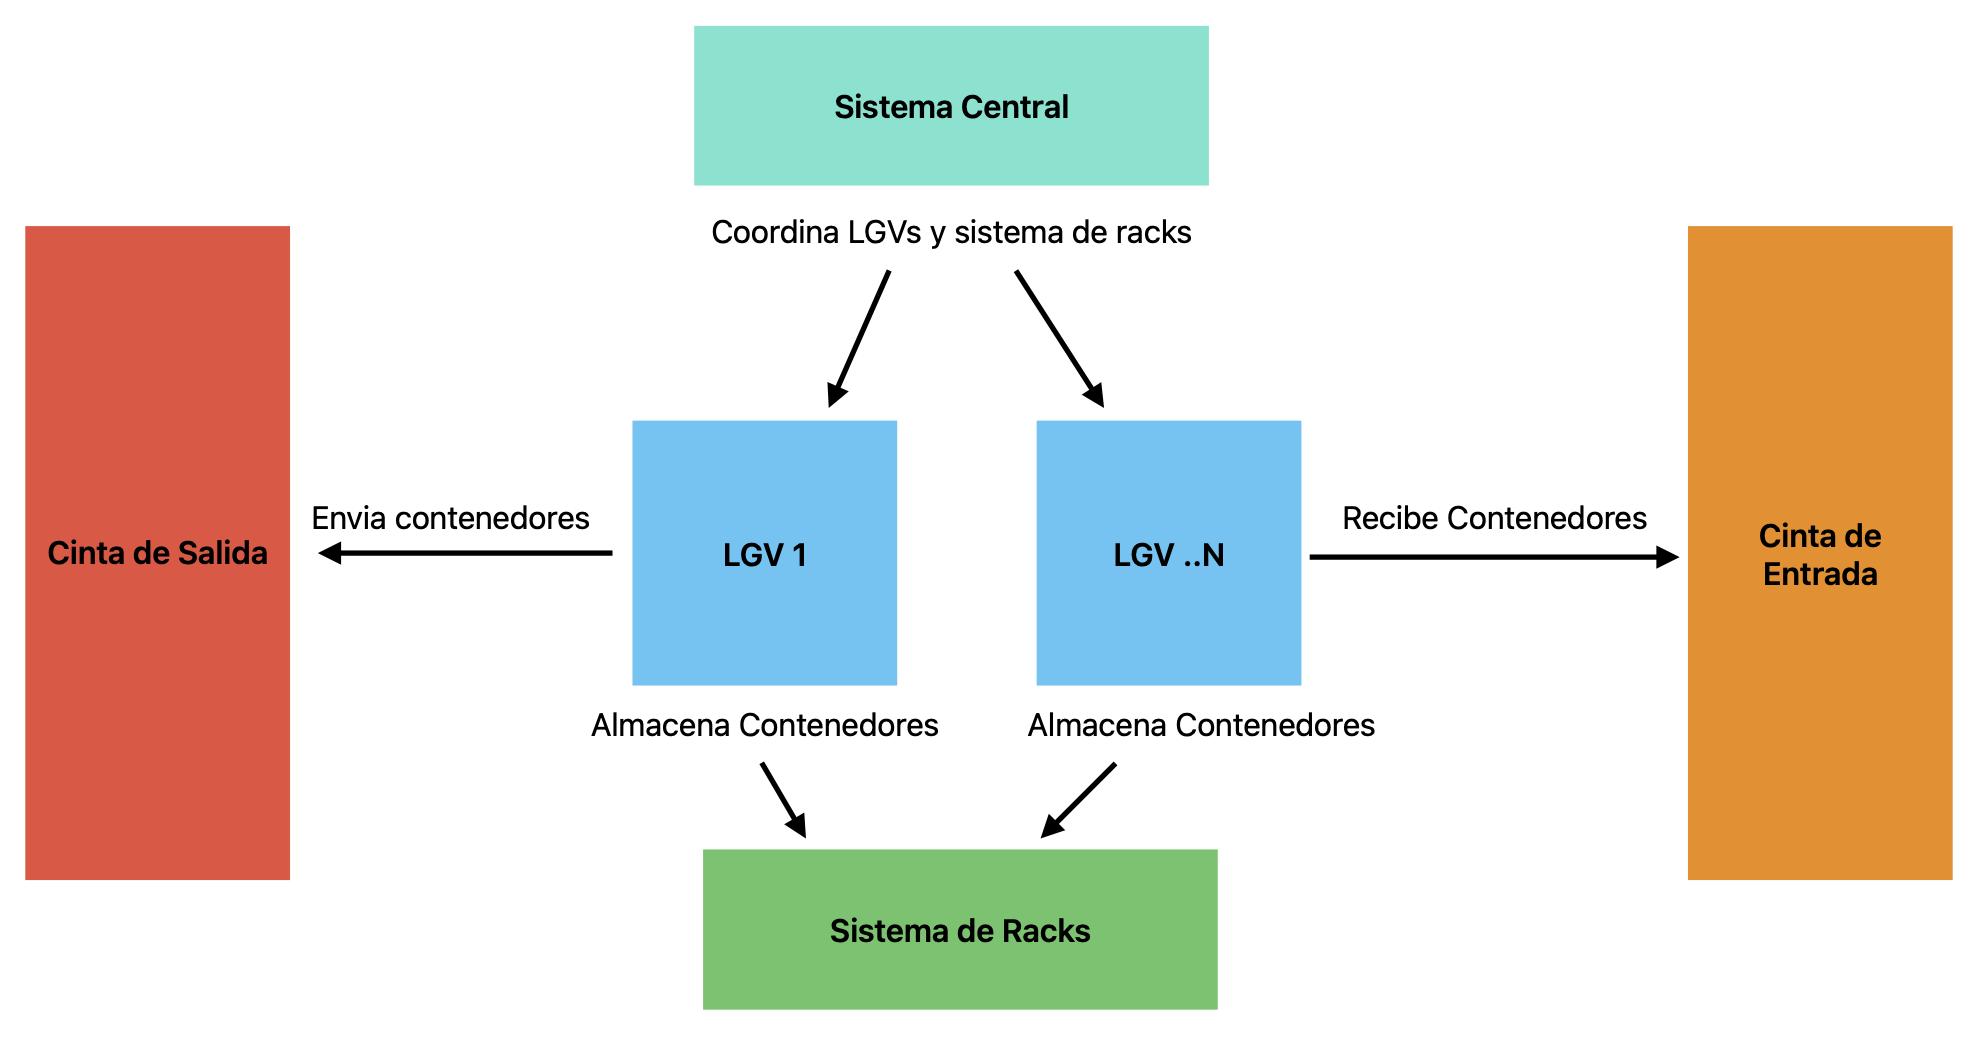
\includegraphics[width=0.5\textwidth]{modeloAgentes.png}
    \caption{Diagrama del modelo de agentes}
    \label{fig:modeloAgentes}
\end{figure}


\subsubsection*{Robots LGV}
\begin{itemize}
    \item Pueden mover pallets en todas las direcciones.
    \item Detección de obstáculos con sensores.
    \item Capacidad para decidir rutas óptimas.
\end{itemize}

\subsubsection*{Sistema de racks}
\begin{itemize}
    \item Almacena los pallets en posiciones específicas.
    \item Capacidad limitada de paquetes por nivel de rack.
\end{itemize}

\subsubsection*{Sistema de carga de batería}
\begin{itemize}
    \item Velocidad de recarga definida.
    \item Permiten cargar los robots cuando bajan de cierto porcentaje de energía.
\end{itemize}

\subsubsection*{Cinta transportadora de entrada}
\begin{itemize}
    \item Introduce pallets al sistema.
\end{itemize}

\subsubsection*{Racks de flujo por gravedad}
\begin{itemize}
    \item Facilitan el flujo de salida.
\end{itemize}

\subsection{Modelo del Entorno}
En la figura 2 se muestra el entorno mapeado utilizando python.
\begin{figure}[h!]
    \centering
    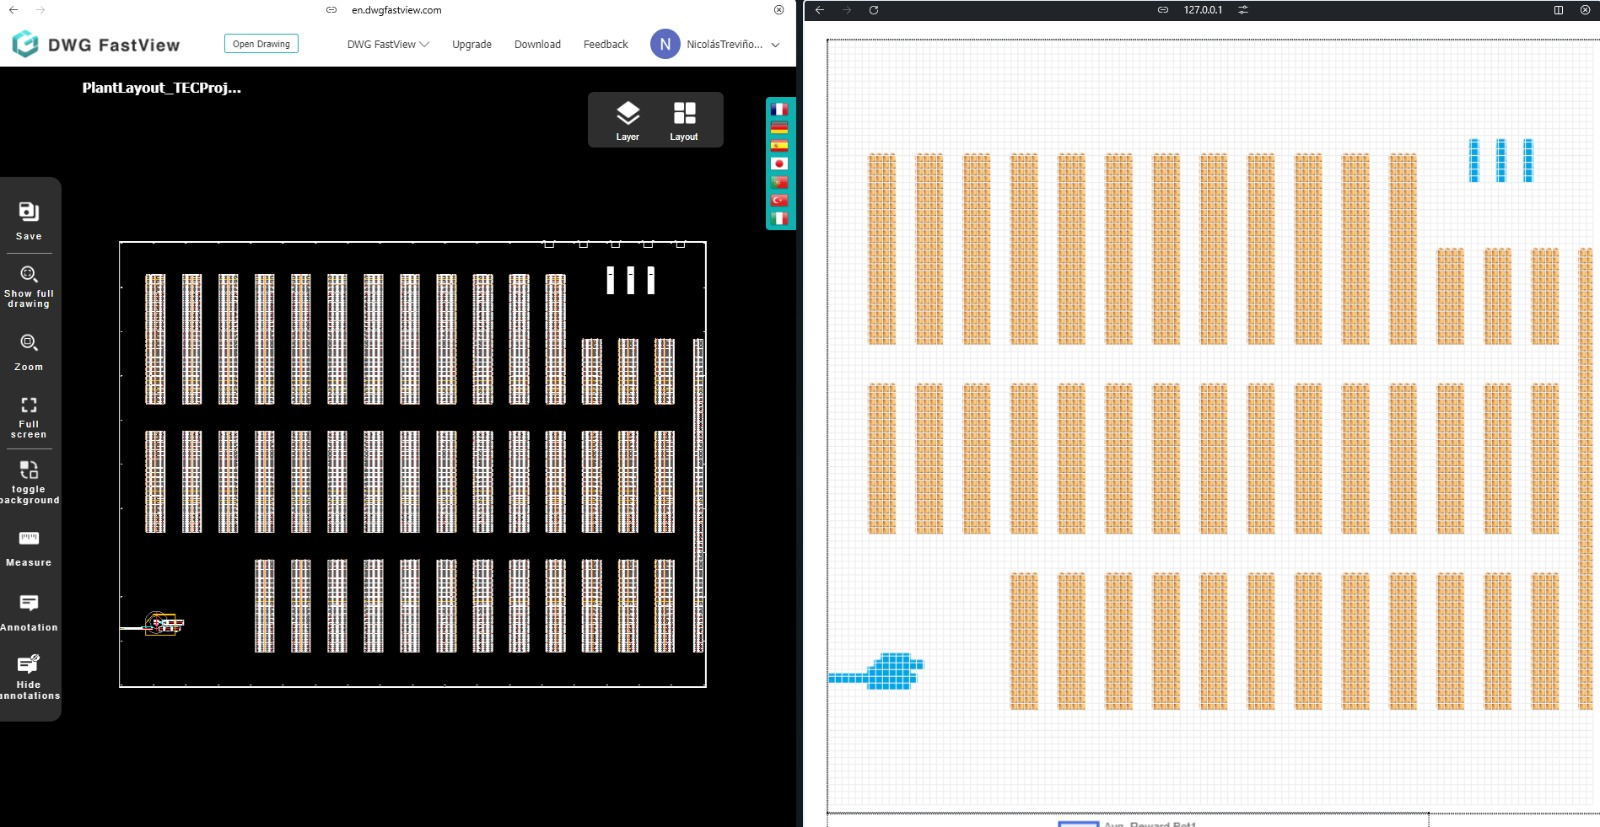
\includegraphics[width=0.5\textwidth]{modeloEntorno.jpeg}
    \caption{Diagrama del modelo del entorno}
    \label{fig:modeloEntorno}
\end{figure}

\subsection{Modelo de la Negociación}
Describa cómo los agentes interactúan, el tipo de mensajes que intercambian, y si se utilizan subastas, votaciones, etc. Incluya un diagrama de comunicaciones.

\subsection{Modelo de la Interacción}
\begin{figure}[h!]
    \centering
    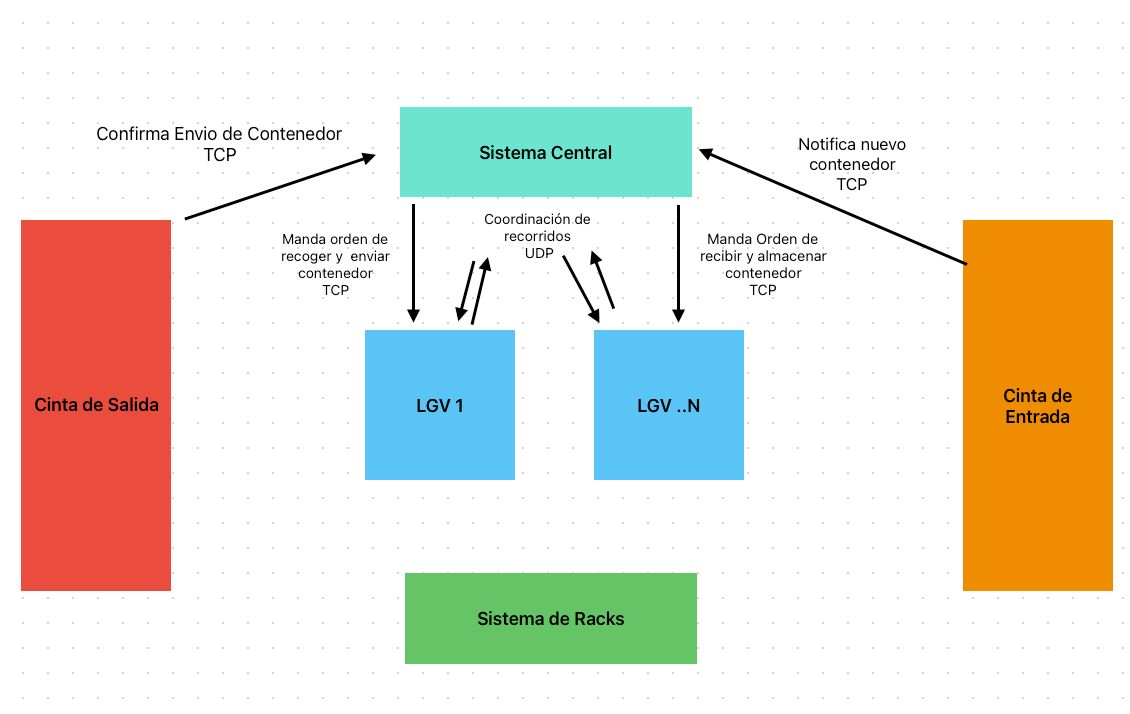
\includegraphics[width=0.5\textwidth]{modeloInteraccion.jpeg}
    \caption{Diagrama de interacción entre los agentes}
    \label{fig:modeloInteraccion}
\end{figure}
\section{Descripción del Modelado Gráfico}
\subsection{Escena a Modelar}
Presente un borrador de la escena a modelar, seguido de la versión final en Unity. Compare las expectativas con el resultado real. No olvide incluir gráficos y ecuaciones que faciliten la interpretación del modelo propuesto.

\section{Algoritmo A*}

Se muestra el Pseudocódigo~\ref{Alg:AstarPseudocodeES} a título de ejemplo de cómo se incluye la descripción de un algoritmo utilizado para dar solución al reto.

\begin{algorithm}[!htb]
\footnotesize
\caption{Algoritmo de Búsqueda A*}
\label{Alg:AstarPseudocodeES}
\begin{algorithmic}[1]
\Require{Grafo $G = (V, E)$, nodo inicial $s$, nodo objetivo $g$, función heurística $h(n)$}
\Ensure{Camino más corto desde $s$ hasta $g$}
    %
    \State{Inicializar la lista abierta $\mathcal{O} \gets \{s\}$}
    \State{Inicializar la lista cerrada $\mathcal{C} \gets \emptyset$}
    \State{Establecer $g(s) \gets 0$, $f(s) \gets h(s)$, y el padre de $s$ como nulo}
    \While{$\mathcal{O} \neq \emptyset$}
        \State{Seleccionar $n \in \mathcal{O}$ como el nodo con el menor $f(n)$}
        \If{$n = g$} 
            \State{\Return Reconstruir el camino desde $s$ hasta $g$}
        \EndIf
        \State{Eliminar $n$ de $\mathcal{O}$ y añadir $n$ a $\mathcal{C}$}
        \For{\textbf{cada} vecino $m$ de $n$}
            \If{$m \in \mathcal{C}$}
                \State{Continuar con el siguiente vecino}
            \EndIf
            \State{Calcular $g(m)$ tentativo $\gets g(n) + \text{coste}(n, m)$}
            \If{$m \notin \mathcal{O}$ o $g(m)$ es menor que el $g(m)$ anterior}
                \State{Asignar el padre de $m$ a $n$}
                \State{Establecer $g(m) \gets g(n) + \text{coste}(n, m)$}
                \State{Establecer $f(m) \gets g(m) + h(m)$}
                \If{$m \notin \mathcal{O}$}
                    \State{Añadir $m$ a $\mathcal{O}$}
                \EndIf
            \EndIf
        \EndFor
    \EndWhile
    \State{\Return{Fracaso, no se encontró ningún camino}}
\Statex

\Procedure{Reconstruir camino}{$g$}
    \State{Inicializar el camino como una lista vacía}
    \State{Establecer el nodo actual como $g$}
    \While{el nodo actual tiene un padre}
        \State{Insertar el nodo actual al inicio del camino}
        \State{Establecer el nodo actual como el padre del nodo actual}
    \EndWhile
    \State{Insertar $s$ al inicio del camino}
    \State{\Return{camino}}
\EndProcedure
\end{algorithmic}
\end{algorithm}

\subsection{Componentes Gráficos}\label{Sec:CompGraf}
\begin{itemize}
    \item \textbf{Nombre del Componente 1}: Breve descripción y fuente. Se debe hacer referencia a su imagen correspondiente en la Figura~\ref{Fi:componente1}
    \begin{figure}[!ht]\centering
	\caption{Componente gráfico 1}\label{Fi:componente1}
    \end{figure}
\end{itemize}

\subsection{Prefabs}
\begin{itemize}
    \item \textbf{Nombre del Prefab}: Breve descripción de la funcionalidad y los scripts utilizados. Utilice el mismo estilo que en la Sección~\ref{Sec:CompGraf}
\end{itemize}

\subsection{Scripts}
Describa cada script y sus interacciones con otros elementos del proyecto. Incluya la fuente si se reutilizó código. Utilice el mismo formato que en el Pseudocódigo~\ref{Alg:AstarPseudocodeES}.

\section{Administración del Proyecto}
\begin{itemize}
    \item Vínculo al Product Backlog
    \item Vínculo al Sprint Backlog
\end{itemize}

\section{Resultados}
Presente los resultados obtenidos en la simulación, comparando con los objetivos propuestos. Incluir gráficos o tablas si es necesario.

\section{Conclusión}
Resuma los principales hallazgos del proyecto y la efectividad de la solución propuesta. Comente posibles mejoras y limitaciones encontradas.

\section{Trabajo Futuro}
Mencione posibles direcciones para continuar el desarrollo del proyecto en el futuro, basándose en las limitaciones observadas.


\bibliographystyle{IEEEtran}
\bibliography{referencias}

\end{document}
